\chapter{QR Factorization}
One algorithmic idea in numerical linear algebra is more important than all the others: QR factorization.

\section{Reduced QR Factorization}
For many applications, we find ourselves interested in the column spaces of a matrix $A$. Note the plural: these are the successive spaces spanned by the columns $a_1, a_2, \ldots$ of $A$ :
\begin{align*}
\left\langle a_1\right\rangle \subseteq\left\langle a_1, a_2\right\rangle \subseteq\left\langle a_1, a_2, a_3\right\rangle \subseteq \cdots
\end{align*}
Here, as in Lecture 5 and throughout the book, the notation $\langle\cdots\rangle$ indicates the subspace spanned by whatever vectors are included in the brackets. Thus $\left\langle a_1\right\rangle$ is the one-dimensional space spanned by $a_1,\left\langle a_1, a_2\right\rangle$ is the two-dimensional space spanned by $a_1$ and $a_2$, and so on. The idea of QR factorization is the construction of a sequence of orthonormal vectors $q_1, q_2, \ldots$ that span these successive spaces.

To be precise, assume for the moment that $A \in \mathbb{C}^{m \times n}(m \geq n)$ has full rank $n$. We want the sequence $q_1, q_2, \ldots$ to have the property
\begin{align*}
\left\langle q_1, q_2, \ldots, q_j\right\rangle=\left\langle a_1, a_2, \ldots, a_j\right\rangle, \quad j=1, \ldots, n .
\end{align*}
From the observations of Lecture 1, it is not hard to see that this amounts to the condition 
\[
    \left[\begin{array}{l|l|l|l}
        & &\\ 
        a_1 & a_2 & \cdots & a_n \\
        & &
        \end{array}\right]=\left[\begin{array}{l|l|l|l} 
        & & & \\
        q_1 & q_2 & \cdots & q_n\\ 
        & & & 
        \end{array}\right]\left[\begin{array}{cccc}
        r_{11} & r_{12} & \cdots & r_{1 n} \\
        & r_{22} & & \vdots \\
        & & \ddots & \vdots \\
        & & & r_{n n}
        \end{array}\right],
\]
where the diagonal entries $r_{kk}$ are nonzero. Written out, these equations take the form
\begin{align*}
\begin{aligned}
& a_1=r_{11} q_1, \\
& a_2=r_{12} q_1+r_{22} q_2, \\
& a_3=r_{13} q_1+r_{23} q_2+r_{33} q_3, \\
& \quad \vdots \\
& a_n=r_{1 n} q_1+r_{2 n} q_2+\cdots+r_{n n} q_n .
\end{aligned}
\end{align*}
As a matrix formula, we have
\begin{align*}
A=\hat{Q} \hat{R},
\end{align*}
where $\hat{Q}$ is $m \times n$ with orthonormal columns and $\hat{R}$ is $n \times n$ and uppertriangular. Such a factorization is called a \textbf{reduced $Q R$ factorization} of $A$.

\section{Full QR Factorization}
A full $Q R$ factorization of $A \in \mathbb{C}^{m \times n}(m \geq n)$ goes further, appending an additional $m-n$ orthonormal columns to $\hat{Q}$ so that it becomes an $m \times m$ unitary matrix $Q$. This is analogous to the passage from the reduced to the full SVD. In the process, rows of zeros are appended to $\hat{R}$ so that it becomes an $m \times n$ matrix $R$, still upper-triangular. The relationship between the full and reduced QR factorizations is as follows.

%────────────────────────────────────────
\begin{figure}[H]
    \centering
    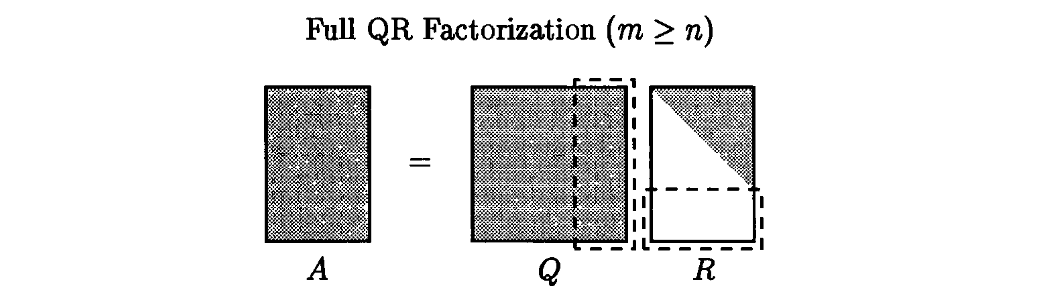
\includegraphics[width=0.8\textwidth]{figures/7-1.png}
\end{figure}
%────────────────────────────────────────

In the full QR factorization, $Q$ is $m \times m, R$ is $m \times n$, and the last $m-n$ columns of $Q$ are multiplied by zeros in $R$ (enclosed by dashes). In the reduced QR factorization, the silent columns and rows are removed. Now $\hat{Q}$ is $m \times n, \hat{R}$ is $n \times n$, and none of the rows of $\hat{R}$ are necessarily zero.

%────────────────────────────────────────
\begin{figure}[H]
    \centering
    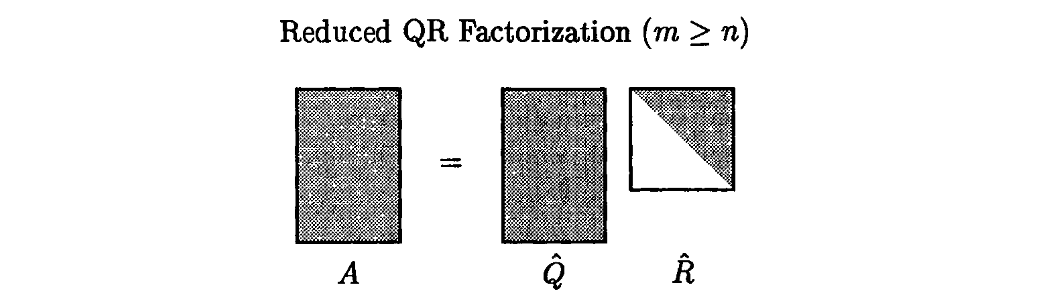
\includegraphics[width=0.8\textwidth]{figures/7-2.png}
\end{figure}
%────────────────────────────────────────

\section{Gram-Schmidt Orthogonalization}
Given $a_1, a_2, \ldots$, we can construct the vectors $q_1, q_2, \ldots$ and entries $r_{i j}$ by a process of successive orthogonalization. This is an old idea, known as GramSchmidt orthogonalization. The process is that: 
\[
    \begin{aligned}
        q_1 & =\frac{a_1}{r_{11}} \\
        q_2 & =\frac{a_2-r_{12} q_1}{r_{22}} \\
        q_3 & =\frac{a_3-r_{13} q_1-r_{23} q_2}{r_{33}} \\
        & \vdots \\
        q_n & =\frac{a_n-\sum_{i=1}^{n-1} r_{i n} q_i}{r_{n n}}. 
        \end{aligned}
\]
where 
\[
    r_{i j}=q_i^* a_j \quad(i \neq j), \quad \left|r_{j j}\right|=\left\|a_j-\sum_{i=1}^{j-1} r_{i j} q_i\right\|_2 .
\]

Note that the sign of $r_{j j}$ is not determined. Arbitrarily, we may choose $r_{j j}>0$, in which case we shall finish with a factorization $A=\hat{Q} \hat{R}$ in which $\hat{R}$ has positive entries along the diagonal. The algorithm is the Gram-Schmidt iteration. Mathematically, it offers a simple route to understanding and proving various properties of QR factorizations. Numerically, it turns out to be unstable because of rounding errors on a computer. To emphasize the instability, numerical analysts refer to this as the classical Gram-Schmidt iteration, as opposed to the modified Gram-Schmidt iteration, discussed in the next lecture.

\begin{algorithm}[H]
    \caption{Classical Gram Schmidt (unstable)}
    \label{Algo 7.1}
    \For{$j=1$ \KwTo $n$}{ 
        $v_j = a_j$\; 
        \For{$i=1$ \KwTo $j-1$}{ 
            $r_{ij} = q_i^*a_j$\; 
            $v_j = v_j - r_{ij}q_i$ \; 
         } 
        $r_{jj} = \|v_j\|_2$\; 
        $q_j = v_j /r_{jj}$\; 
     } 
\end{algorithm}

\section{Existence and Uniqueness} 
All matrices have QR factorizations, and under suitable restrictions, they are unique. We state first the existence result.


%────────────────────────────────────────
\begin{theorem}
\label{thm: Existence of QR}
Every $A \in \mathbb{C}^{m \times n}(m \geq n)$ has a full $Q R$ factorization, hence also a reduced $Q R$ factorization.
\end{theorem}
%────────────────────────────────────────


%────────────────────────────────────────
\begin{theorem}
\label{thm: uniqueness of QR}
Each $A \in \mathbb{C}^{m \times n}(m \geq n)$ of full rank has a unique reduced $Q R$ factorization $A=\hat{Q} \hat{R}$ with $r_{j j}>0$.
\end{theorem}
%───────────────────────────────────────

\section{Solution of $Ax=b$ by QR Factorization} 

In closing this lecture we return for a moment to discrete, finite matrices. Suppose we wish to solve $A x=b$ for $x$, where $A \in \mathbb{C}^{m \times m}$ is nonsingular. If $A=Q R$ is a $Q R$ factorization, then we can write $Q R x=b$, or
\begin{align*}
R x=Q^* b .
\end{align*}
The right-hand side of this equation is easy to compute, if $Q$ is known, and the system of linear equations implicit in the left-hand side is also easy to solve because it is triangular. This suggests the following method for computing the solution to $A x=b$ :
\begin{itemize}
    \item [1.] Compute a QR factorization $A=Q R$.
    \item [2.] Compute $y=Q^* b$.
    \item [3.] Solve $R x=y$ for $x$.
\end{itemize}
In later lectures we shall present algorithms for each of these steps.
The combination 1-3 is an excellent method for solving linear systems of equations; in Lecture 16, we shall prove this. However, it is not the standard method for such problems. Gaussian elimination is the algorithm generally used in practice, since it requires only half as many numerical operations.